\documentclass{standalone}
\usepackage{tikz}
\usetikzlibrary{patterns, positioning}


\begin{document}
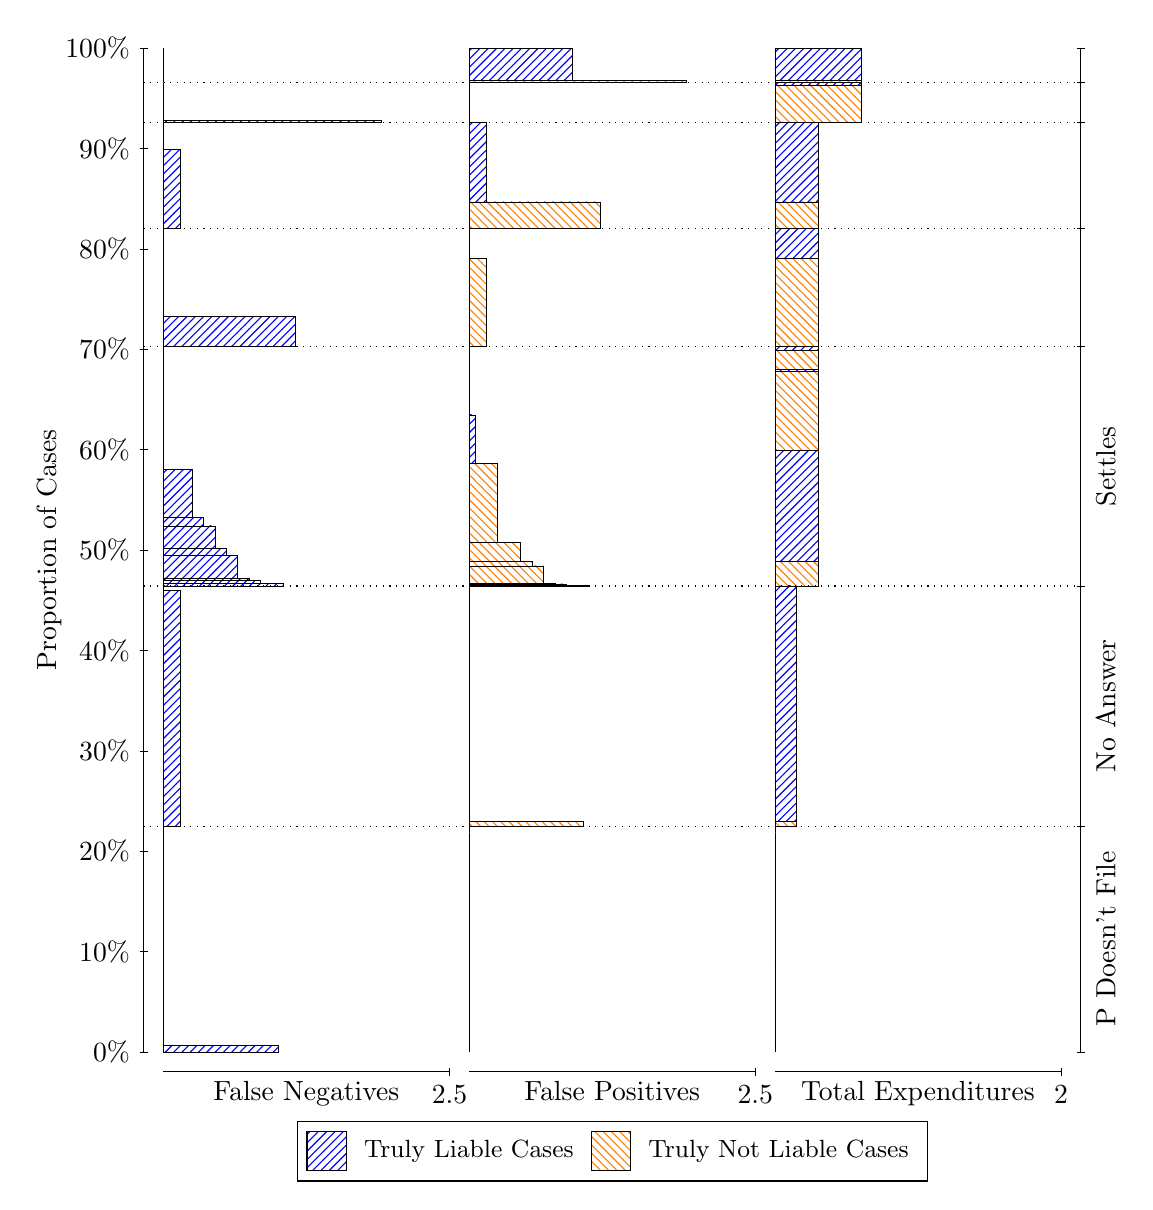
\begin{tikzpicture}
\draw[black, very thin] (1.5,1.75) -- (1.5,14.5);
\node[rotate=90, text=black, anchor=center] at (0.3, 8.125) {Proportion of Cases};
\draw[black, very thin] (1.45,1.75) -- (1.55,1.75);
\node[text=black, anchor=east] at (1.45, 1.75) {0\%};
\draw[black, very thin] (1.45,3.025) -- (1.55,3.025);
\node[text=black, anchor=east] at (1.45, 3.025) {10\%};
\draw[black, very thin] (1.45,4.3) -- (1.55,4.3);
\node[text=black, anchor=east] at (1.45, 4.3) {20\%};
\draw[black, very thin] (1.45,5.575) -- (1.55,5.575);
\node[text=black, anchor=east] at (1.45, 5.575) {30\%};
\draw[black, very thin] (1.45,6.85) -- (1.55,6.85);
\node[text=black, anchor=east] at (1.45, 6.85) {40\%};
\draw[black, very thin] (1.45,8.125) -- (1.55,8.125);
\node[text=black, anchor=east] at (1.45, 8.125) {50\%};
\draw[black, very thin] (1.45,9.4) -- (1.55,9.4);
\node[text=black, anchor=east] at (1.45, 9.4) {60\%};
\draw[black, very thin] (1.45,10.675) -- (1.55,10.675);
\node[text=black, anchor=east] at (1.45, 10.675) {70\%};
\draw[black, very thin] (1.45,11.95) -- (1.55,11.95);
\node[text=black, anchor=east] at (1.45, 11.95) {80\%};
\draw[black, very thin] (1.45,13.225) -- (1.55,13.225);
\node[text=black, anchor=east] at (1.45, 13.225) {90\%};
\draw[black, very thin] (1.45,14.5) -- (1.55,14.5);
\node[text=black, anchor=east] at (1.45, 14.5) {100\%};

\draw[black, very thin] (13.4,1.75) -- (13.4,14.5);
\draw[black, very thin] (13.35,1.75) -- (13.45,1.75);
\node[anchor=west] at (13.35, 1.75) {};
\draw[black, very thin] (13.35,4.6173) -- (13.45,4.6173);
\node[anchor=west] at (13.35, 4.6173) {};
\draw[black, very thin] (13.35,7.6681) -- (13.45,7.6681);
\node[anchor=west] at (13.35, 7.6681) {};
\draw[black, very thin] (13.35,10.711) -- (13.45,10.711);
\node[anchor=west] at (13.35, 10.711) {};
\draw[black, very thin] (13.35,12.206) -- (13.45,12.206);
\node[anchor=west] at (13.35, 12.206) {};
\draw[black, very thin] (13.35,13.553) -- (13.45,13.553);
\node[anchor=west] at (13.35, 13.553) {};
\draw[black, very thin] (13.35,14.06) -- (13.45,14.06);
\node[anchor=west] at (13.35, 14.06) {};
\draw[black, very thin] (13.35,14.5) -- (13.45,14.5);
\node[anchor=west] at (13.35, 14.5) {};

\draw[black, very thin, pattern color=blue, pattern=north east lines] (1.75,1.75) rectangle (3.2033,1.8319);
\draw[black, very thin, pattern color=orange, pattern=north west lines] (1.75,1.8319) rectangle (1.75,4.6173);
\draw[black, very thin, pattern color=blue, pattern=north east lines] (1.75,4.6173) rectangle (1.968,7.6098);
\draw[black, very thin, pattern color=orange, pattern=north west lines] (1.75,7.6098) rectangle (1.75,7.6681);
\draw[black, very thin, pattern color=blue, pattern=north east lines] (1.75,7.6681) rectangle (3.276,7.6968);
\draw[black, very thin, pattern color=blue, pattern=north east lines] (1.75,7.6968) rectangle (3.1307,7.7038);
\draw[black, very thin, pattern color=blue, pattern=north east lines] (1.75,7.7038) rectangle (2.9853,7.7395);
\draw[black, very thin, pattern color=blue, pattern=north east lines] (1.75,7.7395) rectangle (2.84,7.7598);
\draw[black, very thin, pattern color=blue, pattern=north east lines] (1.75,7.7598) rectangle (2.6947,8.0566);
\draw[black, very thin, pattern color=blue, pattern=north east lines] (1.75,8.0566) rectangle (2.5493,8.1411);
\draw[black, very thin, pattern color=blue, pattern=north east lines] (1.75,8.1411) rectangle (2.404,8.4313);
\draw[black, very thin, pattern color=blue, pattern=north east lines] (1.75,8.4313) rectangle (2.2587,8.5386);
\draw[black, very thin, pattern color=blue, pattern=north east lines] (1.75,8.5386) rectangle (2.1133,9.1506);
\draw[black, very thin, pattern color=orange, pattern=north west lines] (1.75,9.1506) rectangle (1.75,10.711);
\draw[black, very thin, pattern color=blue, pattern=north east lines] (1.75,10.711) rectangle (3.4213,11.087);
\draw[black, very thin, pattern color=orange, pattern=north west lines] (1.75,11.087) rectangle (1.75,12.206);
\draw[black, very thin, pattern color=blue, pattern=north east lines] (1.75,12.206) rectangle (1.968,13.212);
\draw[black, very thin, pattern color=orange, pattern=north west lines] (1.75,13.212) rectangle (1.75,13.553);
\draw[black, very thin, pattern color=blue, pattern=north east lines] (1.75,13.553) rectangle (4.5113,13.58);
\draw[black, very thin, pattern color=orange, pattern=north west lines] (1.75,13.58) rectangle (1.75,14.06);
\draw[black, very thin, pattern color=orange, pattern=north west lines] (1.75,14.06) rectangle (1.75,14.091);
\draw[black, very thin, pattern color=blue, pattern=north east lines] (1.75,14.091) rectangle (1.75,14.5);
\draw[black, very thin, pattern color=orange, pattern=north west lines] (5.6333,1.75) rectangle (5.6333,4.5354);
\draw[black, very thin, pattern color=blue, pattern=north east lines] (5.6333,4.5354) rectangle (5.6333,4.6173);
\draw[black, very thin, pattern color=orange, pattern=north west lines] (5.6333,4.6173) rectangle (7.0867,4.6755);
\draw[black, very thin, pattern color=blue, pattern=north east lines] (5.6333,4.6755) rectangle (5.6333,7.6681);
\draw[black, very thin, pattern color=orange, pattern=north west lines] (5.6333,7.6681) rectangle (7.1593,7.6729);
\draw[black, very thin, pattern color=orange, pattern=north west lines] (5.6333,7.6729) rectangle (7.014,7.68);
\draw[black, very thin, pattern color=orange, pattern=north west lines] (5.6333,7.68) rectangle (6.8687,7.6953);
\draw[black, very thin, pattern color=orange, pattern=north west lines] (5.6333,7.6953) rectangle (6.7233,7.7004);
\draw[black, very thin, pattern color=orange, pattern=north west lines] (5.6333,7.7004) rectangle (6.578,7.9246);
\draw[black, very thin, pattern color=orange, pattern=north west lines] (5.6333,7.9246) rectangle (6.4327,7.9814);
\draw[black, very thin, pattern color=orange, pattern=north west lines] (5.6333,7.9814) rectangle (6.4327,7.9833);
\draw[black, very thin, pattern color=orange, pattern=north west lines] (5.6333,7.9833) rectangle (6.2873,8.2179);
\draw[black, very thin, pattern color=orange, pattern=north west lines] (5.6333,8.2179) rectangle (6.142,8.2198);
\draw[black, very thin, pattern color=orange, pattern=north west lines] (5.6333,8.2198) rectangle (5.9967,9.2284);
\draw[black, very thin, pattern color=blue, pattern=north east lines] (5.6333,9.2284) rectangle (5.706,9.8404);
\draw[black, very thin, pattern color=blue, pattern=north east lines] (5.6333,9.8404) rectangle (5.6333,10.711);
\draw[black, very thin, pattern color=orange, pattern=north west lines] (5.6333,10.711) rectangle (5.8513,11.83);
\draw[black, very thin, pattern color=blue, pattern=north east lines] (5.6333,11.83) rectangle (5.6333,12.206);
\draw[black, very thin, pattern color=orange, pattern=north west lines] (5.6333,12.206) rectangle (7.3047,12.546);
\draw[black, very thin, pattern color=blue, pattern=north east lines] (5.6333,12.546) rectangle (5.8513,13.553);
\draw[black, very thin, pattern color=orange, pattern=north west lines] (5.6333,13.553) rectangle (5.6333,14.033);
\draw[black, very thin, pattern color=blue, pattern=north east lines] (5.6333,14.033) rectangle (5.6333,14.06);
\draw[black, very thin, pattern color=orange, pattern=north west lines] (5.6333,14.06) rectangle (8.3947,14.091);
\draw[black, very thin, pattern color=blue, pattern=north east lines] (5.6333,14.091) rectangle (6.9413,14.5);
\draw[black, very thin, pattern color=orange, pattern=north west lines] (9.5167,1.75) rectangle (9.5167,4.5354);
\draw[black, very thin, pattern color=blue, pattern=north east lines] (9.5167,4.5354) rectangle (9.5167,4.6173);
\draw[black, very thin, pattern color=orange, pattern=north west lines] (9.5167,4.6173) rectangle (9.7892,4.6755);
\draw[black, very thin, pattern color=blue, pattern=north east lines] (9.5167,4.6755) rectangle (9.7892,7.6681);
\draw[black, very thin, pattern color=orange, pattern=north west lines] (9.5167,7.6681) rectangle (10.062,7.9814);
\draw[black, very thin, pattern color=blue, pattern=north east lines] (9.5167,7.9814) rectangle (10.062,9.3855);
\draw[black, very thin, pattern color=orange, pattern=north west lines] (9.5167,9.3855) rectangle (10.062,10.394);
\draw[black, very thin, pattern color=blue, pattern=north east lines] (9.5167,10.394) rectangle (10.062,10.423);
\draw[black, very thin, pattern color=orange, pattern=north west lines] (9.5167,10.423) rectangle (10.062,10.661);
\draw[black, very thin, pattern color=blue, pattern=north east lines] (9.5167,10.661) rectangle (10.062,10.711);
\draw[black, very thin, pattern color=orange, pattern=north west lines] (9.5167,10.711) rectangle (10.062,11.83);
\draw[black, very thin, pattern color=blue, pattern=north east lines] (9.5167,11.83) rectangle (10.062,12.206);
\draw[black, very thin, pattern color=orange, pattern=north west lines] (9.5167,12.206) rectangle (10.062,12.546);
\draw[black, very thin, pattern color=blue, pattern=north east lines] (9.5167,12.546) rectangle (10.062,13.553);
\draw[black, very thin, pattern color=orange, pattern=north west lines] (9.5167,13.553) rectangle (10.607,14.033);
\draw[black, very thin, pattern color=blue, pattern=north east lines] (9.5167,14.033) rectangle (10.607,14.06);
\draw[black, very thin, pattern color=orange, pattern=north west lines] (9.5167,14.06) rectangle (10.607,14.091);
\draw[black, very thin, pattern color=blue, pattern=north east lines] (9.5167,14.091) rectangle (10.607,14.5);
\draw[black, dotted] (1.5,4.6173) -- (13.4,4.6173);
\draw[black, dotted] (1.5,7.6681) -- (13.4,7.6681);
\draw[black, dotted] (1.5,10.711) -- (13.4,10.711);
\draw[black, dotted] (1.5,12.206) -- (13.4,12.206);
\draw[black, dotted] (1.5,13.553) -- (13.4,13.553);
\draw[black, dotted] (1.5,14.06) -- (13.4,14.06);
\draw[black, very thin] (1.75,1.5) -- (5.3833,1.5);
\node[text=black, anchor=north] at (3.5667, 1.5) {False Negatives};
\draw[black, very thin] (5.3833,1.45) -- (5.3833,1.55);
\node[text=black, anchor=north] at (5.3833, 1.45) {2.5};

\draw[black, very thin] (5.6333,1.5) -- (9.2667,1.5);
\node[text=black, anchor=north] at (7.45, 1.5) {False Positives};
\draw[black, very thin] (9.2667,1.45) -- (9.2667,1.55);
\node[text=black, anchor=north] at (9.2667, 1.45) {2.5};

\draw[black, very thin] (9.5167,1.5) -- (13.15,1.5);
\node[text=black, anchor=north] at (11.333, 1.5) {Total Expenditures};
\draw[black, very thin] (13.15,1.45) -- (13.15,1.55);
\node[text=black, anchor=north] at (13.15, 1.45) {2};

\node[text=black, centered, rotate=90] at (13.72, 3.1837) {P Doesn't File};
\node[text=black, centered, rotate=90] at (13.72, 6.1427) {No Answer};
\node[text=black, centered, rotate=90] at (13.72, 9.1895) {Settles};





\draw (7.449999999999999,1.5) node[draw=none] (baseCoordinate) {};
\begin{scope}[align=center]
        \matrix[scale=0.5, draw=black, below=0.5cm of baseCoordinate, nodes={draw}, column sep=0.1cm]{
            \node[rectangle, draw, minimum width=0.5cm, minimum height=0.5cm, pattern color=blue, pattern=north east lines] {}; &
            \node[draw=none, font=\small, text=black] (B) {Truly Liable Cases}; &
            \node[rectangle, draw, minimum width=0.5cm, minimum height=0.5cm, pattern color=orange, pattern=north west lines] {}; &
            \node[draw=none, font=\small, text=black] (B) {Truly Not Liable Cases}; \\
            };
\end{scope}

\end{tikzpicture}
\end{document}